% =====================================================================
%  MCMP117 -- Fundamentals of Operating Systems
%  Week 13 Course Notes: Processes & Job Control
%  Compile with XeLaTeX (twice):  xelatex MCMP117_Week13_Notes.tex
%  Needs ./figures/ and the ../code/ folder.
% =====================================================================
\documentclass[11pt,a4paper]{article}
\newcommand{\weeknum}{13}
% ---------- Page & fonts ---------------------------------------------
\usepackage[a4paper,margin=2.3cm,headheight=15pt]{geometry}
\usepackage{fontspec}
\IfFontExistsTF{Calibri}{\setmainfont{Calibri}}{\setmainfont{Carlito}}
\IfFontExistsTF{Cambria}{\newfontfamily\headfont{Cambria}}{\newfontfamily\headfont{Caladea}}
\IfFontExistsTF{Consolas}{\setmonofont[Scale=0.95]{Consolas}}{\setmonofont[Scale=0.88]{DejaVu Sans Mono}}
\usepackage{amsmath,amssymb}
\usepackage{microtype}
\linespread{1.12}
\setlength{\parskip}{0.55em}
\setlength{\parindent}{0pt}

% ---------- Colours (course design system) ----------------------------
\usepackage{xcolor}
\definecolor{dark}{HTML}{212121}
\definecolor{charcoal}{HTML}{36454F}
\definecolor{slate}{HTML}{50808E}
\definecolor{mint}{HTML}{02C39A}
\definecolor{mintdeep}{HTML}{028090}
\definecolor{light}{HTML}{F2F2F2}
\definecolor{muted}{HTML}{6B7679}

% ---------- Packages ---------------------------------------------------
\usepackage{graphicx}
\usepackage{float}
\usepackage{needspace}
\graphicspath{{figures/}}
\usepackage[font=small,labelfont={bf,color=mintdeep},justification=centering]{caption}
\usepackage{booktabs,longtable,array,tabularx}
\usepackage{enumitem}
\setlist{itemsep=0.25em,topsep=0.3em}
\usepackage{tikz}
\usetikzlibrary{arrows.meta,positioning,calc,shapes.geometric}
\usepackage{pgfplots}
\pgfplotsset{compat=1.17}
\usepackage[most]{tcolorbox}
\usepackage{titlesec}
\usepackage{fancyhdr}
\usepackage{xurl}
\usepackage[colorlinks=true,linkcolor=mintdeep,urlcolor=mintdeep,citecolor=mintdeep]{hyperref}

% ---------- Headings ----------------------------------------------------
\titleformat{\section}{\headfont\Large\bfseries\color{charcoal}}{\color{mint}\thesection}{0.7em}{}
\titleformat{\subsection}{\headfont\large\bfseries\color{charcoal}}{\color{mintdeep}\thesubsection}{0.6em}{}
\titleformat{\subsubsection}{\headfont\normalsize\bfseries\color{mintdeep}}{}{0em}{}
\titlespacing*{\section}{0pt}{1.6em}{0.6em}
\titlespacing*{\subsection}{0pt}{1.2em}{0.4em}

% ---------- Header / footer -----------------------------------------------
\pagestyle{fancy}
\fancyhf{}
\fancyhead[L]{\small\color{muted}MCMP117 --- Fundamentals of Operating Systems}
\fancyhead[R]{\small\color{muted}Week \weeknum{} Notes}
\fancyfoot[C]{\small\color{muted}\thepage}
\renewcommand{\headrulewidth}{0pt}

% ---------- Boxes ---------------------------------------------------------
\newtcolorbox{keyidea}[1][Key idea]{enhanced,breakable,colback=charcoal,colframe=charcoal,
  coltext=white,fonttitle=\headfont\bfseries\color{mint},title={#1},
  attach title to upper={\par\smallskip},boxrule=0pt,arc=3pt,left=10pt,right=10pt,top=8pt,bottom=8pt}
\newtcolorbox{example}[1][Worked example]{enhanced,colback=light,colframe=light,
  fonttitle=\headfont\bfseries\color{mintdeep},title={#1},attach title to upper={\par\smallskip},
  boxrule=0pt,arc=3pt,left=10pt,right=10pt,top=8pt,bottom=8pt}
\newtcolorbox{tryit}[1][Try it yourself]{enhanced,breakable,colback=white,colframe=mint,
  fonttitle=\headfont\bfseries\color{mintdeep},title={#1},attach title to upper={\par\smallskip},
  boxrule=0.8pt,arc=3pt,left=10pt,right=10pt,top=8pt,bottom=8pt}
\newtcolorbox{histnote}[1][Historical note]{enhanced,breakable,colback=white,colframe=slate!40,
  fonttitle=\headfont\bfseries\color{slate},title={#1},attach title to upper={\par\smallskip},
  boxrule=0.5pt,arc=3pt,left=10pt,right=10pt,top=8pt,bottom=8pt,fontupper=\small}

% Photo helper: fits image inside a box, never distorted (keepaspectratio)
\newcommand{\photo}[3]{\includegraphics[width=#1,height=#2,keepaspectratio]{#3}}

\newcommand{\term}[1]{\textbf{\color{mintdeep}#1}}
\newcommand{\cmd}[1]{\texttt{#1}}


% ---------- Code listings ----------------------------------------------------
\usepackage{listings}
\lstdefinestyle{course}{
  basicstyle=\ttfamily\small, columns=fullflexible, keepspaces=true,
  backgroundcolor=\color{dark}, rulecolor=\color{dark}, frame=single, framesep=6pt,
  xleftmargin=8pt, xrightmargin=8pt, aboveskip=0.8em, belowskip=0.6em,
  basicstyle=\ttfamily\small\color{light},
  keywordstyle=\color{mint}\bfseries, commentstyle=\color{white!60}\itshape,
  stringstyle=\color{orange!70!yellow}, numberstyle=\tiny\color{muted},
  numbers=left, numbersep=10pt, showstringspaces=false, breaklines=true,
  tabsize=4, upquote=true}
\lstdefinestyle{term}{style=course, numbers=none, keywordstyle=\color{light},
  commentstyle=\color{white!60}, stringstyle=\color{light}}
\lstset{style=course,language=C}
\usepackage{textcomp}

\begin{document}
% ============================ Week 13 body ============================
\lstset{tabsize=8}
% terminal sessions of this week are long: one size smaller than the course default
\lstdefinestyle{wterm}{style=term,basicstyle=\ttfamily\footnotesize\linespread{1.0}\selectfont\color{light},
  literate={─}{{─}}1 {┬}{{┬}}1 {├}{{├}}1 {└}{{└}}1 {│}{{│}}1 {…}{{…}}1}
\thispagestyle{empty}
\begin{tcolorbox}[enhanced,colback=dark,colframe=dark,arc=0pt,boxrule=0pt,
  left=18pt,right=18pt,top=20pt,bottom=20pt,coltext=white]
{\small\color{mint}\textsc{MCMP117 \,·\, Week 13 \,·\, Course Notes}}\par\medskip
{\headfont\fontsize{26}{30}\selectfont\bfseries Fundamentals of Operating Systems}\par\medskip
{\large Processes \& Job Control}\par\smallskip
{\small\itshape\color{white!70} Every command you type becomes a process. This week you learn to watch it, pause it, move it and stop it.}
\end{tcolorbox}

\vspace{0.4em}
{\small
\textbf{Instructor:} Asst.\ Prof.\ Dr.\ (Ph.D.) Hasan Oğuz\\
Head of the Electronical Communication Technology Programme, Vocational School\\
Istanbul Okan University\par}

\vspace{0.8em}
\begin{keyidea}[What you should be able to do after this week]
\begin{enumerate}[leftmargin=1.4em]
  \item Explain how the shell turns every command into a process with \cmd{fork()}, \cmd{exec()} and \cmd{wait()}, and find its PID and PPID.
  \item List and inspect processes with \cmd{ps} (\cmd{-f}, \cmd{-ef}, \cmd{aux}, \cmd{-o}), \cmd{pstree}, \cmd{top}/\cmd{htop} and \texttt{/proc/<pid>/status}, and read every column, including the load average.
  \item Map the five process states of Week~3 to the \texttt{STAT} letters R, S, D, T and Z.
  \item Run jobs in the foreground and background, and move them with \texttt{\&}, Ctrl+Z, Ctrl+C, \cmd{jobs}, \cmd{fg} and \cmd{bg}.
  \item Send signals with \cmd{kill}, \cmd{pkill} and \cmd{killall}; explain SIGTERM, SIGKILL, SIGINT, SIGHUP, SIGSTOP and SIGCONT, and the exit status $128 + n$.
  \item Use \cmd{nohup}, \verb|$$| and \verb|$!|; change priorities with \cmd{nice} and \cmd{renice} and predict CPU shares (Week~5).
  \item Create a zombie process on purpose, recognise it, and explain why only the parent can remove it.
\end{enumerate}
\end{keyidea}

\setcounter{tocdepth}{1}
\tableofcontents

% =====================================================================
\section{From Week 12 to Week 13}

Last week you connected programs with redirections and pipes. Behind every line such as \cmd{grep ERROR logs/system.log | wc -l} the shell quietly created \emph{processes}: two of them, running at the same time, joined by a pipe. This week we look at those processes directly. Almost everything we need was introduced on paper in Week~3 (process, PID, process states, PCB, \cmd{fork()}/\cmd{exec()}/\cmd{wait()}, zombies) and in Week~5 (priority scheduling, nice values). Now you will see each of these ideas in a real Linux terminal and learn to control processes yourself.

\paragraph{About the outputs in these notes.} Every session shown here is real output, captured on our lab machine as the ordinary user \texttt{student} in a freshly created \texttt{\textasciitilde/lab} folder. The commands are in the files \texttt{code/demo\_*.sh} and the captured outputs in \texttt{code/out\_*.txt}. Job control (Ctrl+Z, \cmd{fg}, \cmd{bg}) only works in an \emph{interactive} shell that owns a terminal, so the demos were typed into a real terminal by a small helper program (\texttt{code/record\_session.py}); read the \texttt{demo} files as ``type these lines one by one''. Lines starting with \texttt{\#@} in those files are instructions such as ``press Ctrl+Z''.

On your machine, PIDs, times, dates, terminal names (\texttt{pts/0}) and user numbers will be different, and PIDs change with every run. Listings that contain all processes of the machine (\cmd{ps -ef}, \cmd{ps aux}) have been \emph{trimmed}: we show the first lines and the processes of \texttt{student} only, and cut very long lines with ``\dots''. The order of \cmd{ls} and \cmd{sort} output can depend on the \emph{locale}; we used \cmd{LC\_ALL=C.UTF-8}.

Two harmless test programs appear everywhere this week: \cmd{sleep N} waits $N$ seconds and does nothing (it spends its life in the \emph{waiting} state), and \cmd{yes} prints the letter \texttt{y} forever; with \cmd{yes > /dev/null} its output is thrown away and it simply keeps one CPU core busy (it is always \emph{ready} or \emph{running}).

% =====================================================================
\section{Processes Revisited}
\label{sec:revisit}

Recall from Week~3: a \term{program} is a passive file on disk, such as \texttt{/usr/bin/sleep}; a \term{process} is a program in execution. Each process has a unique \term{process identifier} (PID), knows the PID of its parent (PPID), and is described inside the kernel by its \term{process control block} (PCB). Processes form a tree, because each one (except the first) is created by another.

When you type a command, the shell (\cmd{bash}) does exactly what the Week~3 C program \texttt{fork\_exec\_wait.c} did:
\begin{enumerate}[leftmargin=1.4em]
  \item \cmd{fork()} creates a copy of the shell, the child;
  \item the child calls \cmd{exec()}, which replaces the copy of \cmd{bash} by the program you asked for; the PID stays the same;
  \item the parent shell calls \cmd{wait()} and prints the next prompt only when the child has finished.
\end{enumerate}
If the command ends with \texttt{\&}, step~3 is skipped: the shell does not wait, prints the prompt immediately, and the command runs in the \emph{background}. That is the entire difference between a foreground and a background command.

\begin{figure}[H]
\centering
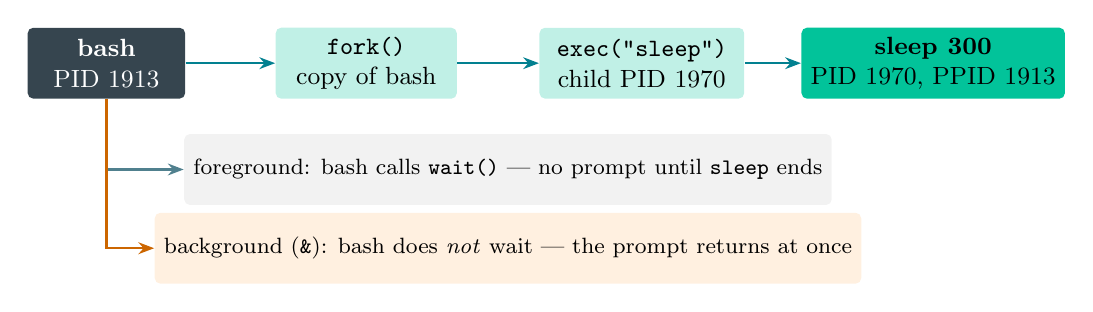
\begin{tikzpicture}[b/.style={rectangle,rounded corners=2pt,minimum height=0.9cm,align=center,font=\small},
  arr/.style={-{Stealth[length=2mm]},thick,mintdeep}]
\node[b,fill=charcoal,text=white,minimum width=2.0cm] (sh) at (0,0) {\textbf{bash}\\PID 1913};
\node[b,fill=mint!25,minimum width=2.3cm] (fk) at (3.3,0) {\texttt{fork()}\\copy of bash};
\node[b,fill=mint!25,minimum width=2.6cm] (ex) at (6.8,0) {\texttt{exec("sleep")}\\child PID 1970};
\node[b,fill=mint,minimum width=2.6cm] (sl) at (10.5,0) {\textbf{sleep 300}\\PID 1970, PPID 1913};
\draw[arr] (sh) -- (fk); \draw[arr] (fk) -- (ex); \draw[arr] (ex) -- (sl);
\node[b,fill=light,minimum width=7.5cm,font=\footnotesize] (fg) at (5.1,-1.35) {foreground: bash calls \texttt{wait()} --- no prompt until \texttt{sleep} ends};
\node[b,fill=orange!12,minimum width=7.5cm,font=\footnotesize] (bg) at (5.1,-2.35) {background (\texttt{\&}): bash does \emph{not} wait --- the prompt returns at once};
\draw[-{Stealth[length=2mm]},slate,thick] (sh.south) |- (fg.west);
\draw[-{Stealth[length=2mm]},orange!80!black,thick] (sh.south) |- (bg.west);
\end{tikzpicture}
\caption{How the shell runs \texttt{sleep 300 \&}. The PIDs are those of the real session in Section~\ref{sec:ps}.}
\end{figure}

% =====================================================================
\section{Looking at Processes}
\label{sec:ps}

\subsection{\texttt{ps}: a snapshot of your processes}

\cmd{ps} (\emph{process status}) prints a one-time snapshot of processes. Without options it shows only the processes attached to your current terminal. \verb|$$| is a special shell variable that holds the PID of the shell itself.

\lstinputlisting[style=wterm,linerange={1-10,17-22}]{../code/out_ps.txt}

What to observe:
\begin{itemize}
  \item Our shell has PID $1913$; it appears in the list as \texttt{bash}, and \cmd{ps -f} shows its full name \texttt{-bash}. The leading dash marks a \emph{login shell}.
  \item \cmd{ps} lists itself: when it takes its snapshot, it is a running process like any other. (After the two background commands, a second plain \cmd{ps}, omitted here, lists \texttt{bash}, \texttt{sleep}, \texttt{yes} and \texttt{ps}.)
  \item The two background commands print \texttt{[1] 1970} and \texttt{[2] 1971}: a \emph{job number} in brackets and the PID.
  \item \cmd{ps -f} (\emph{full format}) adds the owner (UID), the PPID, the CPU usage \texttt{C}, the start time and the whole command line. The PPID of \cmd{sleep} and \cmd{yes} is $1913$: the shell is their parent. The PPID of the shell, $1912$, belongs to the terminal program that started it.
  \item The column \texttt{C} of \cmd{yes} is $96$: it uses almost all of one CPU core. PIDs jump (from $1913$ to $1969$) because other users created processes in the meantime.
\end{itemize}

\subsection{Choosing columns with \texttt{-o}, and \texttt{pstree}}

The option \cmd{-o} lets you choose exactly the columns you need. This is the form we use most often:

\lstinputlisting[style=wterm,firstline=23,lastline=32]{../code/out_ps.txt}

\texttt{STAT} is the process state (Section~\ref{sec:stat}), \texttt{NI} the nice value (Section~\ref{sec:nice}). \cmd{yes} is in state \texttt{R} with $97.4\%$ CPU; \cmd{sleep} is in state \texttt{S} with $0\%$. \cmd{pstree -p \$\$} draws the process tree of Week~3, starting at our shell, with real PIDs: the shell has three children. At the end of the session we stopped both jobs:

% copied verbatim from code/out_ps.txt (listings mis-handles UTF-8 in skipped lines)
\begin{lstlisting}[style=wterm]
student@okan-lab:~/lab$ kill %1 %2
student@okan-lab:~/lab$ jobs
[1]-  Terminated              sleep 300
[2]+  Terminated              yes > /dev/null
\end{lstlisting}

\texttt{\%1} means ``job number 1'' (Section~\ref{sec:jobs}); the shell reports \texttt{Terminated} for each job once.

\subsection{All processes: \texttt{ps -ef}, \texttt{ps aux}, \texttt{ps -u}}

Two option styles exist for historical reasons. \cmd{ps -ef} (System~V style, with a dash) and \cmd{ps aux} (BSD style, \emph{without} a dash) both list \emph{every} process of \emph{every} user; \cmd{aux} adds memory columns. On our lab machine the full lists have about $70$ lines, most of them belonging to \texttt{root}, so we show only the beginning of \cmd{ps -ef} and then select the user \texttt{student} with \cmd{grep} (\cmd{ps -f -u student} gives the same selection in the format of \cmd{ps -f}):

% copied verbatim from code/out_ps.txt (listings mis-handles UTF-8 in skipped lines)
\begin{lstlisting}[style=wterm]
student@okan-lab:~/lab$ ps -ef | head -4
UID        PID  PPID  C STIME TTY          TIME CMD
root         1     0  0 16:17 ?        00:00:02 /process_api --firecracker-init --addr 0.0.0.0:2024 --max-ws-buffer-size 32768 --block-local-connections --listen-vsock-port 2024 --log-vsock-port 5002
root         2     0  0 16:17 ?        00:00:00 [kthreadd]
root         3     2  0 16:17 ?        00:00:00 [pool_workqueue_release]
student@okan-lab:~/lab$ ps aux | head -1
USER       PID %CPU %MEM    VSZ   RSS TTY      STAT START   TIME COMMAND
student@okan-lab:~/lab$ ps aux | grep '^student'
student   1913  0.6  0.0   8436  7532 pts/0    Ss   16:58   0:00 -bash
student   1970  0.0  0.0   3132  1996 pts/0    S    16:58   0:00 sleep 300
student   1971 99.0  0.0   3132  1884 pts/0    R    16:58   0:02 yes
student   1981  0.0  0.0   8340  4328 pts/0    R+   16:58   0:00 ps aux
student   1982  0.0  0.0   4100  2200 pts/0    S+   16:58   0:00 grep ^student
\end{lstlisting}

\begin{itemize}
  \item \textbf{PID 1} is the first user-space process, started by the kernel at boot; it adopts orphans (Week~3). On our lab machine it is a small container start-up program called \texttt{process\_api} (its long command line wraps above); on a normal Ubuntu installation PID~1 is \cmd{systemd}.
  \item \textbf{PID 2}, \texttt{kthreadd}, is the parent of all kernel threads; their names are shown in square brackets.
  \item \cmd{ps aux | grep '\textasciicircum student'} finds the student's lines --- and also the \cmd{grep} process itself, which was running while \cmd{ps} took its snapshot. \cmd{pgrep} (Section~\ref{sec:pkill}) avoids this surprise.
\end{itemize}

\subsection{Reading the columns}

\begin{center}
\renewcommand{\arraystretch}{1.25}
\begin{tabularx}{\linewidth}{>{\ttfamily}l >{\raggedright\arraybackslash}X l}
\toprule
\textbf{\rmfamily Column} & \textbf{Meaning} & \textbf{Example (above)} \\
\midrule
PID, PPID & process ID and parent's process ID (Week 3) & \texttt{1970}, \texttt{1913}\\
UID, USER & owner of the process (Week 11) & \texttt{student}\\
STAT, S & state letter and flags (Section~\ref{sec:stat}) & \texttt{S}, \texttt{R+}, \texttt{Ss}\\
\%CPU, C & CPU time divided by elapsed time since start, in \% & \texttt{99.0} for \cmd{yes}\\
\%MEM & resident memory divided by total RAM, in \% & \texttt{0.0}\\
VSZ & virtual memory size in KiB (Weeks 6--7) & \texttt{3132}\\
RSS & resident set size: the part in RAM, in KiB & \texttt{1884}\\
TTY & terminal of the process; \texttt{?} = none (daemons) & \texttt{pts/0}\\
STIME, START & start time & \texttt{16:58}\\
TIME & total CPU time used so far & \texttt{0:02}\\
CMD, COMMAND & command line (\texttt{[...]} = kernel thread) & \texttt{sleep 300}\\
\bottomrule
\end{tabularx}
\end{center}

\texttt{VSZ} and \texttt{RSS} connect to Weeks~6--7: \cmd{yes} has $3132$~KiB of virtual address space but only $1884$~KiB resident in RAM --- demand paging at work. The \texttt{\%CPU} of \cmd{ps} is an average over the \emph{whole life} of the process; \cmd{top} measures the last few seconds instead. A multithreaded process (Week~4) can show more than $100\%$: $200\%$ means two cores fully busy.

\subsection{Process states in \texttt{ps}: the STAT letters}
\label{sec:stat}

Week~3 described five states: \emph{new}, \emph{ready}, \emph{running}, \emph{waiting} and \emph{terminated}. Linux reports a state letter for each process in the \texttt{STAT} column of \cmd{ps} (the \texttt{S} column of \cmd{top}), and it adds one state that the textbook model does not have: \emph{stopped}.

\begin{figure}[H]
\centering
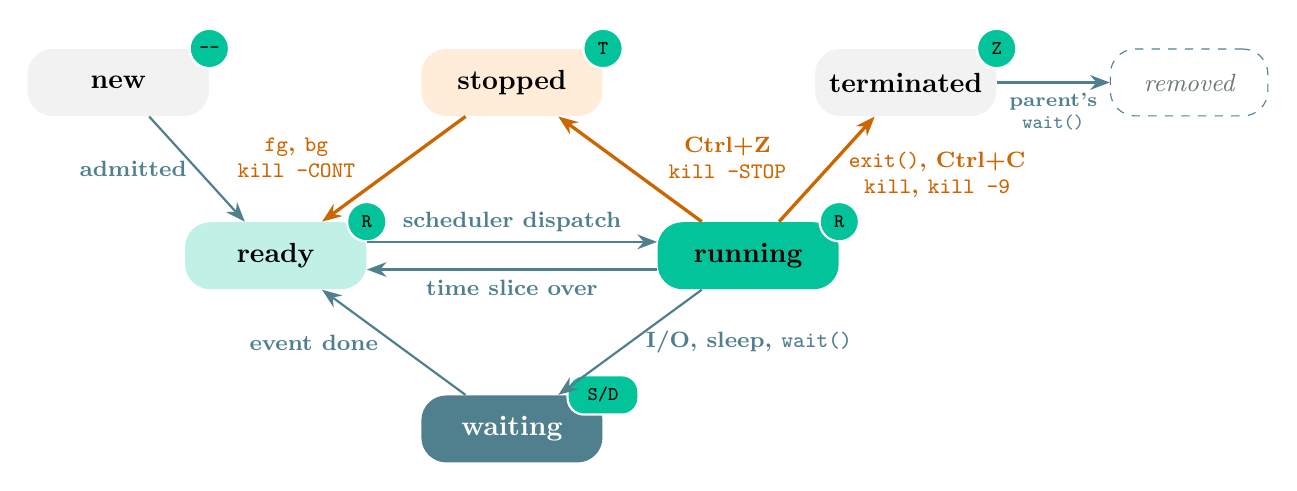
\begin{tikzpicture}[
  st/.style={rectangle,rounded corners=9pt,minimum width=2.3cm,minimum height=0.85cm,font=\headfont\bfseries},
  arr/.style={-{Stealth[length=2.5mm]},thick,slate},
  job/.style={-{Stealth[length=2.5mm]},very thick,orange!80!black},
  lab/.style={font=\footnotesize\bfseries,text=slate},
  jl/.style={font=\footnotesize\bfseries,text=orange!80!black,align=center},
  bd/.style={circle,fill=mint,draw=white,thick,font=\scriptsize\ttfamily\bfseries,inner sep=1.5pt,minimum size=0.5cm}]
\node[st,fill=light] (new) at (0,3) {new};
\node[st,fill=orange!15] (stp) at (5,3) {stopped};
\node[st,fill=light] (trm) at (10,3) {terminated};
\node[st,fill=mint!25] (rdy) at (2,0.8) {ready};
\node[st,fill=mint] (run) at (8,0.8) {running};
\node[st,fill=slate,text=white] (wt) at (5,-1.4) {waiting};
\node[rectangle,rounded corners=9pt,draw=slate,dashed,minimum width=2.0cm,minimum height=0.85cm,font=\itshape\small,text=muted] (gone) at (13.6,3) {removed};
\node[bd] at (new.north east) {--};
\node[bd] at (stp.north east) {T};
\node[bd] at (trm.north east) {Z};
\node[bd] at (rdy.north east) {R};
\node[bd] at (run.north east) {R};
\node[bd,rectangle,rounded corners=6pt,minimum width=0.9cm] at (wt.north east) {S/D};
\draw[arr] (new) -- node[left,lab]{admitted} (rdy);
\draw[arr] ([yshift=5pt]rdy.east) -- node[above,lab]{scheduler dispatch} ([yshift=5pt]run.west);
\draw[arr] ([yshift=-5pt]run.west) -- node[below,lab]{time slice over} ([yshift=-5pt]rdy.east);
\draw[arr] (run) -- node[right,lab,xshift=2pt]{I/O, sleep, \texttt{wait()}} (wt);
\draw[arr] (wt) -- node[left,lab,xshift=-2pt]{event done} (rdy);
\draw[job] (run) -- node[right,jl,xshift=10pt,yshift=4pt]{Ctrl+Z\\\texttt{kill -STOP}} (stp);
\draw[job] (stp) -- node[left,jl,xshift=-10pt,yshift=4pt]{\texttt{fg}, \texttt{bg}\\\texttt{kill -CONT}} (rdy);
\draw[job] (run) -- node[right,jl,xshift=4pt,yshift=-2pt]{\texttt{exit()}, Ctrl+C\\\texttt{kill}, \texttt{kill -9}} (trm);
\draw[arr] (trm) -- node[below,lab,font=\scriptsize\bfseries,align=center]{parent's\\\texttt{wait()}} (gone);
\end{tikzpicture}
\caption{The Week~3 state diagram with the \texttt{STAT} letter of each state (mint badges) and the job-control actions of this week (orange arrows). Grey arrows are taken by the kernel and the scheduler.}
\label{fig:states}
\end{figure}

\begin{center}
\renewcommand{\arraystretch}{1.25}
\begin{tabularx}{\linewidth}{>{\ttfamily\bfseries}c >{\raggedright\arraybackslash}X >{\raggedright\arraybackslash}p{3.0cm} >{\raggedright\arraybackslash}p{3.2cm}}
\toprule
\textbf{\rmfamily Letter} & \textbf{Meaning} & \textbf{Week 3 state} & \textbf{Seen in these notes}\\
\midrule
R & running or runnable: on a CPU, or in the ready queue & running \emph{or} ready & \cmd{yes > /dev/null}\\
S & interruptible sleep: waiting for an event (timer, keyboard, child) & waiting & \cmd{sleep}, \cmd{bash}\\
D & uninterruptible sleep, usually waiting for disk I/O & waiting & rare and short\\
T & stopped by Ctrl+Z or SIGSTOP & (Linux extra) & Section~\ref{sec:jobs}\\
Z & zombie: terminated, exit status not yet collected & terminated & Section~\ref{sec:zombie}\\
\bottomrule
\end{tabularx}
\end{center}

Characters after the letter are \emph{flags}: \texttt{s} = session leader (your login shell shows \texttt{Ss}), \texttt{+} = member of the foreground process group (\cmd{ps} itself shows \texttt{R+}), \texttt{N} = low priority, i.e.\ positive nice value (\texttt{RN}, \texttt{SN}), \texttt{<} = high priority, \texttt{l} = multithreaded. Three remarks:
\begin{itemize}
  \item Linux does not distinguish \emph{ready} from \emph{running}: both are \texttt{R}. On a machine with $2$ cores at most $2$ processes are really running at any instant; the other \texttt{R} processes are in the ready queue.
  \item The \emph{new} state lasts only microseconds and has no letter.
  \item A process in state \texttt{S} can also be killed: \cmd{sleep} spends its whole life in \texttt{S}, and we kill it all the time. The diagram draws the \cmd{kill} arrow from \emph{running} only to stay readable.
\end{itemize}

\subsection{\texttt{/proc/<pid>/status}: the PCB as text}
\label{sec:proc}

Since Week~3 we know that Linux shows parts of every PCB as text files under \texttt{/proc}. \verb|$!| is the PID of the most recent background job:

\Needspace{10\baselineskip}
\lstinputlisting[style=wterm,linerange={1-15,21-24}]{../code/out_proc.txt}

The fields map onto the PCB of Week~3: \texttt{State} (\texttt{S}, waiting for its timer), \texttt{Pid} and \texttt{PPid} (identity and parent), \texttt{Uid} (the owner's user number; $1013$ on our lab machine, typically $1000$ on yours, Week~11), \texttt{VmRSS} (memory-management information), \texttt{Threads} (Week~4) and the context-switch counters (accounting information: a \emph{voluntary} switch happens when the process gives up the CPU to wait, a \emph{nonvoluntary} one when the scheduler takes the CPU away). (The full session in \texttt{code/out\_proc.txt} also reads \texttt{/proc/\$!/cmdline} and the links \texttt{cwd} and \texttt{exe}: the command line, the current directory and the program file.) Our own shell (\verb|$$|) is also sleeping: it waits for the keyboard.

\subsection{\texttt{top} and \texttt{htop}: the live view}
\label{sec:top}

\cmd{top} shows the processes sorted by CPU usage and refreshes every few seconds; press \texttt{q} to quit. To print it in these notes we used \emph{batch mode} (\cmd{-b}) with one iteration (\cmd{-n 1}) and the user filter \cmd{-u student}, while a \cmd{yes} and a \cmd{sleep} (started with \texttt{\&} half a minute earlier) were running:

\lstinputlisting[style=wterm,firstline=5,lastline=21]{../code/out_top.txt}

\begin{itemize}
  \item \textbf{Line 1} (the same as the output of \cmd{uptime}): current time, time since boot, number of logged-in users ($0$ on our lab machine because nobody is logged in on its console) and the \term{load average} for the last $1$, $5$ and $15$ minutes.
  \item \textbf{Line 2} counts all tasks of the machine by state: running ($R$), sleeping ($S$ and $D$), stopped ($T$), zombie ($Z$).
  \item \textbf{Line 3} splits the CPU time of the \emph{whole machine}: \texttt{us} user mode, \texttt{sy} kernel mode (dual mode, Week~2), \texttt{ni} niced user processes, \texttt{id} idle, \texttt{wa} waiting for I/O, \texttt{st} ``stolen'' by the virtualisation host. One busy core out of $2$ is only $1/2 = 50\%$ of the machine.
  \item \textbf{Lines 4--5}: memory and swap in MiB (Weeks~6--7).
  \item \textbf{Process list}: \texttt{PR} is the priority, $\text{PR} = 20 + \text{NI}$ for normal processes; \texttt{VIRT}/\texttt{RES} are virtual and resident memory; \texttt{S} is the state; \texttt{\%CPU} is measured over the last refresh interval. \cmd{yes} uses $100\%$ of \emph{one} core.
\end{itemize}

Useful keys in \cmd{top}: \texttt{P} sort by CPU, \texttt{M} sort by memory, \texttt{u} show one user, \texttt{k} kill (asks for a PID and a signal), \texttt{r} renice, \texttt{1} show every CPU, \texttt{q} quit. \cmd{htop} is a friendlier, coloured version: select a process with the arrow keys, \texttt{F9} sends a signal, \texttt{F7}/\texttt{F8} change the nice value, \texttt{F10} quits. Install it with \cmd{sudo apt install htop} if it is missing.

\begin{example}[Reading the load average]
The load average counts processes that are running or ready (state R), plus those in uninterruptible disk wait (D), averaged over $1$, $5$ and $15$ minutes. It only makes sense relative to the number of cores $c$ (\cmd{nproc} prints it; $c = 2$ on our lab machine):
\begin{align*}
\text{load } 0.59: &\quad 0.59 / 2 = 29.5\% \text{ of the capacity is used,}\\
\text{load } 2.00: &\quad 2.00 / 2 = 100\%: \text{ every core is busy, nobody waits,}\\
\text{load } 3.00: &\quad 3.00 / 2 = 150\%: \text{ on average } 3 - 2 = 1 \text{ process waits in the ready queue.}
\end{align*}
If the $1$-minute value is above the $15$-minute value, the load is rising. Our snapshot was taken $30$~s after \cmd{yes} started, so the $1$-minute average ($0.59$) had not yet climbed to $1$: the averages are exponentially decaying, not instant counts. In \texttt{/proc/loadavg}, the fourth field \texttt{3/98} means $3$ runnable tasks now out of $98$, and the last number is the most recently assigned PID. In Week~4 terms: a load above $c$ means processes spend time in the ready queue, so their waiting time grows. (Numbers checked with \texttt{code/check\_numbers.py}.)
\end{example}

% =====================================================================
\section{Job Control}
\label{sec:jobs}

A \term{job} is one command line started by the shell: a single process, or several processes connected by pipes. The shell numbers its jobs \texttt{[1]}, \texttt{[2]}, \dots{} Only \emph{one} job at a time owns the keyboard: the \term{foreground} job. The keys Ctrl+C and Ctrl+Z send signals (Section~\ref{sec:signals}) to the foreground job only. Any number of jobs can run in the \term{background}.

In the \textbf{foreground} (\texttt{command}) the shell waits and shows no prompt until the job ends; the job reads the keyboard; Ctrl+C terminates it and Ctrl+Z stops it. Use it for short commands and interactive programs (\cmd{nano}, \cmd{less}, \cmd{top}). In the \textbf{background} (\texttt{command \&}) the shell prints \texttt{[job] PID} and the prompt at once; keys do not reach the job (use \cmd{kill \%n}); if it tries to read the keyboard it is stopped (\texttt{Stopped (tty input)}); its output still appears on the terminal unless you redirect it (Week~12). Use it for long, non-interactive work: compiling, copying, downloads.

\subsection{Stopping a job with Ctrl+Z, continuing it with \texttt{bg}}

\lstinputlisting[style=wterm,firstline=1,lastline=19]{../code/out_jobs.txt}

\begin{enumerate}[leftmargin=1.4em]
  \item \cmd{sleep 100} runs in the foreground: no prompt. Pressing \textbf{Ctrl+Z} (echoed as \texttt{\^{}Z}) stops it; the shell reports \texttt{[1]+ Stopped} and gives the prompt back.
  \item \cmd{jobs} lists the jobs of this shell; \cmd{ps} shows the state \texttt{T} (stopped). A stopped process keeps its memory and open files but receives no CPU time: in Week~3 terms it is neither ready nor waiting, which is why Linux needs the extra state.
  \item \cmd{bg} lets the current job continue in the \emph{background}; the shell prints the command with an \texttt{\&} added. \cmd{jobs -l} adds the PIDs. \cmd{sleep} is back in state \texttt{S}: it is waiting for its timer again, not stuck.
\end{enumerate}

\subsection{Starting with \texttt{\&}, \texttt{fg}, Ctrl+C and \texttt{kill \%n}}

\lstinputlisting[style=wterm,firstline=20,lastline=38]{../code/out_jobs.txt}

\begin{itemize}
  \item \texttt{[3] 2405}: job number $3$, PID $2405$. In the \cmd{jobs} list, \texttt{+} marks the \emph{current} job (the default for \cmd{fg} and \cmd{bg} without an argument) and \texttt{-} the previous one.
  \item \cmd{fg \%3} brings \cmd{yes} to the foreground (the shell prints its command line); \textbf{Ctrl+C} (\texttt{\^{}C}) terminates it.
  \item \cmd{kill \%1 \%2} sends SIGTERM to jobs $1$ and $2$. The shell reports \texttt{Terminated} once, just before the next prompt; the second \cmd{jobs} prints nothing.
\end{itemize}

\subsection{Naming jobs and processes; \texttt{\$\$} and \texttt{\$!}}

\begin{center}
\renewcommand{\arraystretch}{1.2}
\begin{tabularx}{\linewidth}{>{\ttfamily}l >{\raggedright\arraybackslash}X >{\ttfamily}l}
\toprule
\textbf{\rmfamily You write} & \textbf{It means} & \textbf{\rmfamily Example}\\
\midrule
\%1, \%2, \dots & job number $n$ of this shell & fg \%2, kill \%1\\
\%+ \textrm{or} \%\% & the current job (marked \texttt{+}) & fg\\
\%- & the previous job (marked \texttt{-}) & bg \%-\\
\%sleep & the job whose command starts with \texttt{sleep} & kill \%sleep\\
1970 & a PID: valid in every terminal and for every tool & kill 1970\\
\$\$ & PID of the current shell & echo \$\$\\
\$! & PID of the most recent background job & kill \$!\\
\bottomrule
\end{tabularx}
\end{center}

Job numbers exist only inside the shell that started the jobs: a second terminal has its own \texttt{[1]}. PIDs are global. \textbf{Careful:} \cmd{kill 1} (without \texttt{\%}) means PID~$1$, not job~$1$ --- see the common errors in Section~\ref{sec:errors}. The variables \verb|$$| and \verb|$!| will be useful in Week~14 scripts.

% =====================================================================
\section{Signals}
\label{sec:signals}

\subsection{What a signal is}

A \term{signal} is a small, numbered notification that the kernel delivers to a process. It is the software counterpart of the hardware interrupt of Week~2: an interrupt makes the CPU stop what it is doing and run a handler; a signal makes one \emph{process} stop what it is doing and react. Signals are sent by users (keys, the \cmd{kill} command), by other processes, and by the kernel itself (for example SIGCHLD when a child terminates, SIGSEGV after an illegal memory access).

The kernel marks the signal as pending and delivers it to the target process, which reacts in one of three ways: the \emph{default action} of that signal (terminate, stop, continue, or ignore), a \emph{handler} function of its own (\emph{catching} the signal), or ignoring it. Two signals are special: \textbf{SIGKILL (9)} and \textbf{SIGSTOP (19)} can be neither caught nor ignored --- the kernel acts alone. Ordinary users may signal only their own processes; \texttt{root} may signal any (a protection rule, Week~11).

\begin{histnote}[Why ``kill'' and ``hang up''?]
In early UNIX the command that sends signals was named \cmd{kill} because the default action of most signals is to terminate the process; the name stayed even though \cmd{kill -STOP} or \cmd{kill -CONT} kill nothing. SIGHUP (``hang up'') comes from the time when terminals were connected through telephone lines and modems: when the line was hung up, the processes of that session received SIGHUP. Today closing a terminal window or an SSH connection does the same.
\end{histnote}

\subsection{The signal table}
\label{sec:sigtable}

\cmd{kill -l} lists all $64$ signal numbers of Linux (first lines below; the full list is in \texttt{code/out\_signals.txt}). \cmd{kill -l 15} converts a number to a name, \cmd{kill -l KILL} a name to a number.

\lstinputlisting[style=wterm,firstline=1,lastline=4]{../code/out_signals.txt}

\begin{center}
\renewcommand{\arraystretch}{1.25}
\begin{tabularx}{\linewidth}{c >{\ttfamily}l >{\raggedright\arraybackslash}X >{\raggedright\arraybackslash}p{3.2cm} c}
\toprule
\textbf{No.} & \textbf{\rmfamily Name} & \textbf{Sent by} & \textbf{Default action} & \textbf{Catchable?}\\
\midrule
1 & SIGHUP & closing the terminal or SSH session & terminate & yes\\
2 & SIGINT & Ctrl+C & terminate & yes\\
3 & SIGQUIT & Ctrl+\textbackslash & terminate + core dump & yes\\
9 & SIGKILL & \cmd{kill -9}: the last resort & terminate at once & \textbf{no}\\
11 & SIGSEGV & the kernel, after an illegal memory access (Week~7) & terminate + core dump & yes\\
15 & SIGTERM & \cmd{kill} (default), \cmd{pkill}, \cmd{killall}, system shutdown & terminate & yes\\
17 & SIGCHLD & the kernel, when a child terminates or stops & ignore & yes\\
18 & SIGCONT & \cmd{fg}, \cmd{bg}, \cmd{kill -CONT} & continue if stopped & yes\\
19 & SIGSTOP & \cmd{kill -STOP} & stop & \textbf{no}\\
20 & SIGTSTP & Ctrl+Z & stop & yes\\
\bottomrule
\end{tabularx}
\end{center}
The numbers are those of Linux on x86 and ARM; some differ on other UNIX systems, so names are safer than numbers (except $9$ and $15$, which are the same everywhere). You may write the name with or without the prefix: \cmd{kill -TERM}, \cmd{kill -SIGTERM} and \cmd{kill -15} are equivalent.

\subsection{SIGTERM, SIGKILL, SIGINT and the exit status}

\lstinputlisting[style=wterm,firstline=19,lastline=32]{../code/out_signals.txt}

The built-in command \cmd{wait \$!} waits for the background job to end and makes the shell report \emph{how} it ended: \texttt{Terminated} (SIGTERM), \texttt{Killed} (SIGKILL) or \texttt{Interrupt} (SIGINT: a third experiment with \cmd{kill -INT}, in the full output file, prints \texttt{Interrupt}). Then \verb|$?|, the exit status of the last command, encodes the signal:

\begin{keyidea}[Exit status of a process killed by a signal]
If a process is terminated by signal number $n$, the shell sets its exit status to $128 + n$:
\[
\text{SIGTERM: } 128 + 15 = 143, \qquad \text{SIGKILL: } 128 + 9 = 137, \qquad \text{SIGINT: } 128 + 2 = 130 .
\]
A normal exit gives a status between $0$ and $127$ (usually $0$ for success). Conversely, a status $s > 128$ means ``killed by signal $s - 128$''.
\end{keyidea}

\subsection{Pausing and resuming: SIGSTOP and SIGCONT}

\lstinputlisting[style=wterm,firstline=40,lastline=52]{../code/out_signals.txt}

\cmd{kill -STOP} puts \cmd{sleep} into state \texttt{T} --- exactly the state that Ctrl+Z produces, which is why the shell reports the job as \texttt{Stopped}. \cmd{kill -CONT} lets it continue (\texttt{S} again). This is what \cmd{fg} and \cmd{bg} do internally: they send SIGCONT.

\subsection{Choosing processes by name: \texttt{pgrep}, \texttt{pkill}, \texttt{killall}}
\label{sec:pkill}

\lstinputlisting[style=wterm,firstline=53,lastline=71]{../code/out_signals.txt}

\cmd{pgrep} prints the PIDs of processes whose name matches a pattern (\cmd{-l} adds the name, \cmd{-c} counts them); \cmd{pkill} sends them a signal (SIGTERM by default); \cmd{killall} does the same with an exact program name. The last \cmd{pgrep} finds nothing, and its exit status is $1$. \textbf{Always add \cmd{-u student}} (your own user name): without it these tools also try to signal other users' processes, which fails with ``Operation not permitted'' --- and, run as root, would actually kill them. Test the pattern with \cmd{pgrep} before using \cmd{pkill}: \cmd{pkill -u student bash} would close all your terminals.

\subsection{Catching signals: \texttt{catch.c}}

A program can install its own \emph{handler} for most signals. The program \texttt{code/catch.c} catches SIGINT and SIGTERM, and also tries --- and fails --- to install a handler for SIGKILL. The listing shows its core; the complete file adds the \texttt{\#include} lines, the \texttt{struct sigaction} set-up and the start-up message:

\lstinputlisting[caption={}]{../code/catch_excerpt.c}

Compiled with \cmd{gcc -Wall -O2} (no warnings) and run in \texttt{\textasciitilde/lab/src}:

\lstinputlisting[style=wterm,firstline=1,lastline=24]{../code/out_catch.txt}

The installation of a SIGKILL handler fails (\texttt{Invalid argument}): the kernel refuses it. Ctrl+C and \cmd{kill -INT} no longer terminate the program --- the handler runs and the program carries on. Ctrl+Z still stops it (SIGTSTP is not caught) and \cmd{bg} continues it. SIGTERM makes it clean up and exit normally (\cmd{jobs} reports \texttt{Done}, not \texttt{Terminated}), and \cmd{kill -9} always works (\texttt{Killed}).
Messages printed by a background job appear wherever the cursor is --- right after the prompt --- so the next command you type starts on a new line. This looks odd, but it is normal.

\subsection{Stopping a process safely}

\begin{keyidea}[Ask first, force last]
\begin{enumerate}[leftmargin=1.4em]
  \item Foreground job: press Ctrl+C (SIGINT).
  \item Otherwise: \cmd{kill PID} (SIGTERM) and wait $5$--$10$ seconds.
  \item Check with \cmd{ps -p PID} whether it is still there, and in which state.
  \item Only then: \cmd{kill -9 PID} (SIGKILL).
\end{enumerate}
\end{keyidea}

\textbf{Warning about \cmd{kill -9}.} SIGKILL gives the program no chance to save open documents, flush buffers or delete temporary and lock files; a database may need repair afterwards, and the program's children are not informed. And sometimes \cmd{kill -9} does not help at all: a zombie (\texttt{Z}) is already dead (Section~\ref{sec:zombie}); a process in state \texttt{D} receives the signal only when its disk I/O finishes; and another user's process cannot be signalled (``Operation not permitted'').

\subsection{SIGHUP and \texttt{nohup}}
\label{sec:nohup}

When you close a terminal (or an SSH connection), the shell's jobs receive SIGHUP and, by default, terminate. \cmd{nohup command} starts a command that ignores SIGHUP. In this session we simulate closing the terminal with \cmd{kill -HUP}:

\lstinputlisting[style=wterm,firstline=1,lastline=23]{../code/out_nohup.txt}

The plain \cmd{sleep 500} ended (\texttt{Hangup}), the two \cmd{nohup} jobs kept running. If the output of a \cmd{nohup} command goes to the terminal, \cmd{nohup} redirects it to the file \texttt{nohup.out} (and says so: the message appeared after the prompt because the background \cmd{nohup} printed it a moment later). The clean form is
\begin{lstlisting}[style=term]
nohup long_command > run.log 2>&1 &
\end{lstlisting}
which uses the redirections of Week~12. Typical use: start a long job on a remote server over SSH, log out, and look at \texttt{run.log} later.

% =====================================================================
\section{Priorities: \texttt{nice} and \texttt{renice}}
\label{sec:nice}

In Week~5 we met priority scheduling and the Linux scheduler, which shares the CPU among runnable processes in proportion to a \emph{weight}. The weight comes from the \term{nice value}, an integer from $-20$ to $+19$ ($40$ values, default $0$). As in Week~5, a \emph{smaller} number means a \emph{higher} priority: a process with a high nice value is ``nice'' to the others. \cmd{top} shows the priority $\text{PR} = 20 + \text{NI}$.



\lstinputlisting[style=wterm,firstline=1,lastline=28]{../code/out_nice.txt}

\begin{itemize}
  \item \cmd{nice} without arguments prints the current nice value, $0$. \cmd{nice -n 10 command} starts a command with nice value $10$; \cmd{ps} shows \texttt{NI 10} and the flag \texttt{N} (\texttt{RN}).
  \item \cmd{renice -n 15 -p PID} changes the value of a running process. \cmd{renice} calls it ``priority'' in its message; it is the nice value. Raising it ($10 \to 15$) is allowed; lowering it again ($15 \to 5$) is \texttt{Permission denied} for ordinary users --- otherwise everybody would set $-20$. \cmd{nice -n -5} prints a warning and runs the command at nice $0$.
  \item The last experiment repeats the Week~5 measurement with \cmd{yes}: two CPU-bound processes are pinned to the same core with \cmd{taskset -c 1} (without pinning, each would get its own core and both would show about $100\%$).
\end{itemize}

\begin{example}[Predicting the CPU shares]
The kernel's weight for nice $0$ is $1024$, for nice $10$ it is $110$ (each nice step changes the weight by a factor of about $1.25$, and $1.25^{10} \approx 9.31$). Two CPU-bound processes on one core get
\[
\frac{1024}{1024 + 110} \approx 90.3\,\%, \qquad \frac{110}{1024 + 110} \approx 9.7\,\%, \qquad \text{ratio } \frac{1024}{110} \approx 9.31 .
\]
We measured $89.3\%$ and $9.6\%$, a ratio of $89.3 / 9.6 \approx 9.30$. (The two values do not add up to exactly $100\%$ because \cmd{ps} averages over each process's lifetime and the two did not start at exactly the same moment. Numbers checked with \texttt{code/check\_numbers.py}.)
\end{example}

As \texttt{root}, \cmd{sudo renice -n -5 -p PID} would work (Week~11) --- but on a shared machine, do not give your own processes priority over everyone else's.

% =====================================================================
\section{Zombies and Orphans, Made Visible}
\label{sec:zombie}

Week~3 defined a \term{zombie} as a process that has terminated but whose parent has not yet collected its exit status with \cmd{wait()}. The kernel has already freed its memory and closed its files; only the process-table entry with the PID and the exit status remains. In Week~3 we produced one with a shell trick; now we write the smallest possible C program that does it on purpose, \texttt{code/zombie.c}:

\lstinputlisting[caption={}]{../code/zombie_excerpt.c}

The listing shows the heart of the program; the complete file adds the \texttt{\#include} lines, reads \texttt{secs} from the command line (default $30$) and checks for a failed \cmd{fork()}. The child exits at once with status $7$; the parent sleeps for \texttt{secs} seconds \emph{without} calling \cmd{wait()}, then reaps the child with \cmd{waitpid()}. We copied \texttt{zombie.c} into \texttt{\textasciitilde/lab/src} and ran:

\lstinputlisting[style=wterm,firstline=1,lastline=28]{../code/out_zombie.txt}

\begin{itemize}
  \item PID $3120$, the child, is in state \texttt{Z}, its name is shown in brackets and marked \texttt{<defunct>}; its parent is $3119$. \texttt{/proc} agrees: \texttt{State: Z (zombie)}. (\cmd{pgrep -n} selects the \emph{newest} matching process, which is the child.)
  \item \cmd{kill -9} on the zombie does \emph{nothing}: you cannot kill what is already dead.
  \item The shell's \cmd{wait} waits for the background job \texttt{./zombie}; after $25$ seconds the parent calls \cmd{waitpid()}, receives the exit status $7$, and the zombie disappears from the list.
\end{itemize}

A few zombies are harmless. A buggy parent that creates children in a loop and never waits for them can, however, fill the process table: PIDs are limited (\nolinkurl{/proc/sys/kernel/pid_max} is $32768$ on our machine, so the largest PID is $32767$), and then no new process can be created. The cure is to fix or end the \emph{parent}: when the parent terminates, the zombie becomes an \term{orphan}, is adopted by PID~$1$ (or a ``subreaper'' process), and that new parent reaps it at once (Week~3). The kernel helps parents with the signal SIGCHLD, sent when a child terminates; a well-written parent reacts to it by calling \cmd{wait()}.

% =====================================================================
\section{Command Reference}

{\small
\renewcommand{\arraystretch}{1.18}
\noindent\begin{tabularx}{\linewidth}{@{}>{\ttfamily\raggedright\arraybackslash}p{3.85cm} >{\raggedright\arraybackslash}X @{\hspace{8pt}} >{\ttfamily\raggedright\arraybackslash}p{3.85cm} >{\raggedright\arraybackslash}X@{}}
\toprule
\multicolumn{2}{@{}l}{\textbf{Inspecting}} & \multicolumn{2}{l@{}}{\textbf{Job control}}\\
\midrule
ps \textrm{/} ps -f & this terminal (short/full) & cmd \& & start in the background\\
ps -ef \textrm{/} ps aux & all processes & Ctrl+C \textrm{/} Ctrl+Z & SIGINT / SIGTSTP to the foreground job\\
ps -u student & one user's processes & jobs \textrm{/} jobs -l & list jobs (with PIDs)\\
ps -o pid,stat,cmd & choose the columns & fg \%n \textrm{/} bg \%n & to the foreground / continue in the background\\
ps -p PID & one process & wait [\%n] & wait for a background job\\
ps --sort=-\%cpu & highest CPU first & & \\
\midrule
\multicolumn{2}{@{}l}{\textbf{Inspecting (cont.)}} & \multicolumn{2}{l@{}}{\textbf{Signals}}\\
\midrule
pstree -p [PID] & process tree with PIDs & kill PID \textrm{/} kill \%n & SIGTERM (15)\\
pgrep -u student -l name & PIDs and names (\texttt{-c} count, \texttt{-n} newest) & kill -INT \textrm{/} -HUP \textrm{/} -9 & SIGINT, SIGHUP, SIGKILL\\
top \textrm{/} htop & live view (q quits) & kill -STOP \textrm{/} -CONT & pause / resume\\
uptime \textrm{/} nproc & load average / cores & kill -l [n] & list signals / number to name\\
cat /proc/PID/status & the PCB as text & pkill -u student pat & signal by name pattern\\
echo \$\$ \textrm{/} echo \$! & PID of shell / last background job & killall -u student name & signal by exact name\\
\midrule
\multicolumn{2}{@{}l}{\textbf{Priority}} & \multicolumn{2}{l@{}}{\textbf{Surviving logout}}\\
\midrule
nice -n 10 cmd & start with nice value 10 & nohup cmd > log 2>\&1 \& & ignore SIGHUP, output to \texttt{log}\\
renice -n 15 -p PID & change it (users: only upwards) & taskset -c 1 cmd & run on core 1 only (experiments)\\
\bottomrule
\end{tabularx}
}

% =====================================================================
\section{Common Errors and What They Mean}
\label{sec:errors}

\begin{description}[leftmargin=0pt,itemsep=0.35em]
  \item[\texttt{-bash: kill: (1) - Operation not permitted}] You typed \cmd{kill 1} and meant job~$1$. Without \texttt{\%} the number is a PID, and PID~$1$ belongs to root. Use \cmd{kill \%1}. (Real output, Lab Sheet solution B4.)
  \item[\texttt{-bash: kill: \%6: no such job}] There is no job $6$ in \emph{this} shell. Check with \cmd{jobs}; jobs from another terminal must be addressed by PID.
  \item[\texttt{renice: failed to set priority for ... Permission denied}] An ordinary user tried to lower a nice value. Only raising is allowed.
  \item[\texttt{nice: cannot set niceness: Permission denied}] A negative nice value as an ordinary user. The command runs anyway, at nice $0$.
  \item[\texttt{pkill: killing pid ... failed: Operation not permitted}] The pattern also matched another user's process. Add \cmd{-u} with your user name.
  \item[The prompt does not come back] A foreground job is running (you forgot the \texttt{\&}). Press Ctrl+C to end it, or Ctrl+Z and then \cmd{bg} to keep it running in the background.
  \item[\texttt{[1]+ Stopped (tty input)}] A background job wanted to read the keyboard (try \cmd{nano \&} or \cmd{cat \&}). Bring it to the foreground with \cmd{fg}.
  \item[\texttt{There are stopped jobs.}] You typed \cmd{exit} while jobs are stopped. Resume or kill them (\cmd{jobs}, \cmd{fg}, \cmd{kill \%n}); typing \cmd{exit} a second time exits anyway, and the stopped jobs are terminated.
  \item[A \texttt{Z <defunct>} line survives \cmd{kill -9}] A zombie is already dead. Only a \cmd{wait()} by its parent removes it; end or fix the parent.
  \item[\texttt{grep} appears in its own result] A pipeline such as \cmd{ps aux | grep sleep} also lists the \cmd{grep} process itself. Use \cmd{pgrep -l sleep} instead.
\end{description}

% =====================================================================
\section{Summary}

\begin{keyidea}[Week 13 in eight sentences]
\begin{enumerate}[leftmargin=1.4em]
  \item Every command is a process created by the shell with \cmd{fork()} and \cmd{exec()}; in the foreground the shell \cmd{wait()}s, with \texttt{\&} it does not.
  \item \cmd{ps} (\cmd{-f}, \cmd{-ef}, \cmd{aux}, \cmd{-o}) and \cmd{pstree} take snapshots; \cmd{top}/\cmd{htop} give a live view; \texttt{/proc/<pid>/status} shows the PCB.
  \item STAT letters: R = ready or running, S/D = waiting, T = stopped (a Linux extra), Z = terminated but not yet reaped.
  \item The load average counts processes that want a CPU; compare it with the number of cores.
  \item Ctrl+Z stops the foreground job, \cmd{bg} and \cmd{fg} continue it, \cmd{jobs} lists jobs; \texttt{\%n} names a job, a plain number a PID.
  \item \cmd{kill} sends signals (default SIGTERM, 15); Ctrl+C sends SIGINT (2); SIGKILL (9) and SIGSTOP (19) cannot be caught; a process killed by signal $n$ has exit status $128 + n$.
  \item \cmd{nohup} protects a job from SIGHUP; \cmd{nice}/\cmd{renice} set the nice value $-20 \dots 19$, which users may only raise; nice $10$ against nice $0$ gets about $1/9.3$ of the CPU.
  \item A zombie cannot be killed; only its parent's \cmd{wait()} (or the parent's death and adoption by PID~1) removes it.
\end{enumerate}
\end{keyidea}

% =====================================================================
\section{Glossary}

\begin{description}[leftmargin=0pt,itemsep=0.15em]
  \item[Background job] A job started with \texttt{\&}; the shell does not wait for it.
  \item[Foreground job] The one job that receives keyboard input and the signals of Ctrl+C and Ctrl+Z.
  \item[Job] A command line started by the shell (one or more processes), numbered \texttt{[1]}, \texttt{[2]}, \dots
  \item[Load average] Average number of processes running, ready or in disk wait over $1$, $5$ and $15$ minutes.
  \item[Nice value] Number from $-20$ to $19$ that sets a process's CPU weight; higher is ``nicer'' (lower priority).
  \item[Orphan] A process whose parent has terminated; adopted by PID~1.
  \item[Signal] Numbered software notification delivered by the kernel to a process.
  \item[SIGKILL / SIGTERM] Signal 9 (cannot be caught, immediate termination) / signal 15 (polite request to terminate).
  \item[Stopped (T)] State of a process paused by SIGTSTP or SIGSTOP; continued by SIGCONT.
  \item[Zombie (Z)] A terminated process whose exit status has not yet been collected by its parent.
\end{description}

% =====================================================================
\section{Try It Yourself}

\begin{tryit}[Processes on your own machine]
\textbf{Linux} (lab PCs, WSL, or a virtual machine), in \texttt{\textasciitilde/lab}; compile the two programs with \cmd{gcc -Wall -O2 -o zombie zombie.c} and \cmd{gcc -Wall -O2 -o catch catch.c}.
\begin{enumerate}[leftmargin=1.4em]
  \item Start \cmd{top} in one terminal and \cmd{yes > /dev/null \&} three times in another. Watch the load average climb over a minute. Which value does it approach?
  \item Run \cmd{nano notes.txt}, press Ctrl+Z, run \cmd{ls}, then \cmd{fg}. Your text is still there.
  \item Change \texttt{catch.c} so that it also catches SIGTSTP. What happens now when you press Ctrl+Z?
  \item Run \cmd{./zombie 60 \&}, find the zombie, then kill the \emph{parent} with \cmd{kill PID}. What happens to the zombie, and why?
\end{enumerate}
\end{tryit}

% =====================================================================
\section{Review Questions}

\subsection*{Conceptual}
\begin{enumerate}[leftmargin=1.6em]
  \item What does the shell do differently for \cmd{sleep 10} and \cmd{sleep 10 \&}? Use the words \cmd{fork()}, \cmd{exec()} and \cmd{wait()}.
  \item Map each of the five Week~3 states to the letters that \cmd{ps} shows. Which Linux state has no Week~3 counterpart?
  \item What is the difference between \cmd{kill 3} and \cmd{kill \%3}?
  \item Compare SIGTERM and SIGKILL. Why should SIGTERM be tried first? In which situations does even SIGKILL not remove a process from the list?
  \item What do \cmd{fg} and \cmd{bg} send to a stopped job, and what is the difference between them?
  \item Why may an ordinary user raise but not lower a nice value?
\end{enumerate}

\subsection*{Numerical}
\begin{enumerate}[leftmargin=1.6em,resume]
  \item A job ended and \verb|echo $?| prints $130$. What happened? What would $129$ and $137$ mean?
  \item A machine with $4$ cores shows \texttt{load average: 6.00, 3.00, 1.00}. Interpret each value. Is the load rising or falling?
  \item Two CPU-bound processes share one core; one has nice $0$ (weight $1024$), the other nice $5$ (weight $335$). Compute their CPU shares.
  \item A process in \cmd{top} shows \texttt{NI 19}. What is its \texttt{PR}? What is the \texttt{PR} of a process with nice $-20$?
  \item A shell has four jobs. The commands \cmd{sleep 50 \&}, \cmd{sleep 60 \&}, \cmd{sleep 70} (then Ctrl+Z) were typed in this order after \cmd{yes > /dev/null \&}. Which job number does each have, and what is the current job?
\end{enumerate}

\subsection*{Answers to the numerical questions}
\begin{enumerate}[leftmargin=1.6em,start=7]
  \item $130 = 128 + 2$: terminated by SIGINT (Ctrl+C). $129 = 128 + 1$: SIGHUP (hang-up). $137 = 128 + 9$: SIGKILL.
  \item Relative to $4$ cores: last minute $6/4 = 150\%$ (on average $6 - 4 = 2$ processes waiting for a CPU); last $5$ minutes $3/4 = 75\%$; last $15$ minutes $1/4 = 25\%$. The $1$-minute value is the largest: the load is rising.
  \item $1024/(1024 + 335) = 1024/1359 \approx 75.3\%$ and $335/1359 \approx 24.7\%$; ratio $1024/335 \approx 3.06 \approx 1.25^{5} \approx 3.05$.
  \item $\text{PR} = 20 + 19 = 39$; for nice $-20$: $\text{PR} = 20 - 20 = 0$.
  \item \cmd{yes} is \texttt{[1]}, \cmd{sleep 50} \texttt{[2]}, \cmd{sleep 60} \texttt{[3]}, \cmd{sleep 70} \texttt{[4]} (stopped). The current job (\texttt{+}) is the most recently stopped or started one, \texttt{[4]}; \texttt{[3]} is marked \texttt{-}.
\end{enumerate}

% =====================================================================
\section{Looking Ahead: Week 14}

Next week we put commands into files and turn them into programs: \textbf{Introduction to Shell Scripting}. You will write scripts with a shebang line, make them executable with \cmd{chmod +x}, and use variables, quoting, command substitution \verb|$( )|, arithmetic \verb|$(( ))|, positional parameters, \cmd{read}, the exit status \verb|$?|, tests, \texttt{if}, loops and functions. This week's material returns at once: \verb|$$| and \verb|$!| to manage background jobs, \cmd{wait} to wait for them, and the $128 + n$ rule when a script checks why a command failed. Week~15 is the final exam review.

\subsection*{Further reading (optional)}
\begin{itemize}
  \item A.\ Silberschatz, P.\,B.\ Galvin and G.\ Gagne, \emph{Operating System Concepts}, 10th ed., Wiley: Chapter~3 (Processes), in particular Sections~3.1--3.3 (process concept, scheduling, operations on processes), and Section~5.7 on Linux scheduling (nice values).
  \item R.\,H.\ and A.\,C.\ Arpaci-Dusseau, \emph{Operating Systems: Three Easy Pieces}:
  \begin{itemize}
    \item Chapter~4, ``The Abstraction: The Process'': \url{https://pages.cs.wisc.edu/~remzi/OSTEP/cpu-intro.pdf}
    \item Chapter~5, ``Interlude: Process API'' (fork, exec, wait, signals, \cmd{ps}, \cmd{top}, \cmd{kill}): \url{https://pages.cs.wisc.edu/~remzi/OSTEP/cpu-api.pdf}
  \end{itemize}
  \item The GNU Bash manual, section ``Job Control'': \url{https://www.gnu.org/software/bash/manual/html_node/Job-Control.html}
\end{itemize}

% =====================================================================
\section{Lab Sheet}
\label{sec:lab}

\textbf{Preparation:} \cmd{bash mcmp117\_lab\_setup.sh} then \cmd{cd \textasciitilde/lab}. Copy \texttt{zombie.c} from the Week~13 \texttt{code/} folder into \texttt{\textasciitilde/lab/src}. Use only \cmd{sleep} and \cmd{yes} as test processes and replace \texttt{student} by your own user name. For every exercise, write down the command line(s) and the relevant output, and answer the question. Points in brackets, $100$ in total. Solutions are in Section~\ref{sec:sol}; try first!

\subsection*{Part A --- Inspecting processes (26 points)}
\begin{enumerate}[leftmargin=2.2em,label=\textbf{A\arabic*}]
  \item {[4]} Print the PID of your shell and find the same number in the output of \cmd{ps}.
  \item {[5]} Run \cmd{ps -f}. Which PPID does the \cmd{ps} process have, and why is it equal to \verb|$$|?
  \item {[6]} Start \cmd{sleep 1000 \&}. Using \texttt{/proc/\$!/status}, report its \texttt{State} and \texttt{PPid}. Which Week~3 state is this?
  \item {[5]} Start two more \cmd{sleep} jobs and draw the tree that \cmd{pstree -p \$\$} prints.
  \item {[6]} Start \cmd{yes > /dev/null \&} and show \texttt{pid}, \texttt{stat} and \texttt{cmd} of all processes of this terminal. Explain why \cmd{yes} is \texttt{R} and \cmd{sleep} is \texttt{S}.
\end{enumerate}

\subsection*{Part B --- Job control (24 points)}
\begin{enumerate}[leftmargin=2.2em,label=\textbf{B\arabic*}]
  \item {[6]} Run \cmd{sleep 500} in the foreground and stop it with Ctrl+Z. Show it with \cmd{jobs} and show its \texttt{STAT} with \cmd{ps}.
  \item {[6]} Continue the job of B1 in the background. Prove with \cmd{jobs -l} and \cmd{ps} that it runs again.
  \item {[6]} Start three \cmd{sleep} jobs in the background. Bring job~$2$ to the foreground and end it with Ctrl+C. What does \cmd{jobs} show now?
  \item {[6]} Type \cmd{kill 1}, then \cmd{kill \%1}. Explain the two different results.
\end{enumerate}

\subsection*{Part C --- Signals (26 points)}
\begin{enumerate}[leftmargin=2.2em,label=\textbf{C\arabic*}]
  \item {[8]} End three \cmd{sleep 300 \&} jobs with SIGTERM, SIGKILL and SIGINT respectively. After each one, run \cmd{wait \$!} and \cmd{echo \$?}. Explain the three numbers.
  \item {[6]} Pause a background \cmd{sleep} with \cmd{kill -STOP} and resume it with \cmd{kill -CONT}; show \texttt{STAT} after each step.
  \item {[6]} Start \cmd{sleep 901}, \cmd{sleep 902} and \cmd{sleep 903} in the background. Count your \cmd{sleep} processes with \cmd{pgrep}, terminate all of them with one command, and count again.
  \item {[6]} Start \cmd{sleep 800 \&} and \cmd{nohup sleep 900 > /dev/null 2>\&1 \&}. Send SIGHUP to both jobs. Which one survives, and why?
\end{enumerate}

\subsection*{Part D --- Priority, zombies and challenges (24 points)}
\begin{enumerate}[leftmargin=2.2em,label=\textbf{D\arabic*}]
  \item {[7]} Start \cmd{sleep 600} with nice value $15$ and check \texttt{NI} and \texttt{STAT}. Raise its nice value to $19$, then try to set it back to $0$. Explain the result.
  \item {[8]} Compile \texttt{zombie.c} with \cmd{gcc -Wall -O2}, run \cmd{./zombie 30 \&} and show the zombie with \cmd{ps}. Try \cmd{kill -9} on it. What happens, and what finally removes it?
  \item {[4]} \emph{Challenge.} With one command line, show your three processes with the highest \texttt{\%CPU} (plus the header line).
  \item {[5]} \emph{Challenge (Week~12).} With one pipeline, count how many of your processes are in each state (first letter of \texttt{STAT}).
\end{enumerate}

% =====================================================================
\section{Lab Sheet Solutions}
\label{sec:sol}

The solutions were run in a freshly created lab. Outputs that already appeared in the tutorial sections are referenced; the others (A3, A5, B4, C3, D1, D3, D4) come from \texttt{code/demo\_lab.sh}, whose complete real output is in \texttt{code/out\_lab.txt}. Your PIDs will differ. Other correct solutions exist; what counts is the right result and a sensible explanation.

{\footnotesize
\renewcommand{\arraystretch}{1.2}
\begin{longtable}{@{}p{0.6cm}>{\raggedright\arraybackslash}p{7.3cm}>{\raggedright\arraybackslash}p{7.6cm}@{}}
\toprule
& \textbf{Command line(s)} & \textbf{Expected output / answer}\\
\midrule
\endhead
\textbf{A1} & \texttt{echo \$\$}\newline \texttt{ps} & A number such as \texttt{1913}; the line with that PID in \cmd{ps} is \texttt{bash} (Section~\ref{sec:ps}).\\
\textbf{A2} & \texttt{ps -f} & The PPID of \texttt{ps -f} equals the shell's PID: the shell forked the process that became \cmd{ps}.\\
\textbf{A3} & \texttt{sleep 1000 \&}\newline \texttt{grep -E '\textasciicircum(State|PPid)' /proc/\$!/status} & \texttt{State: S (sleeping)}, \texttt{PPid:} the shell's PID (\texttt{3207} in \texttt{out\_lab.txt}). Week~3 state: \emph{waiting} (for a timer).\\
\textbf{A4} & \texttt{sleep 2000 \& sleep 3000 \&}\newline \texttt{pstree -p \$\$} & \texttt{bash(PID)} with the children \texttt{pstree}, and three \texttt{sleep} processes, as in Section~\ref{sec:ps}.\\
\textbf{A5} & \texttt{yes > /dev/null \&}\newline \texttt{ps -o pid,stat,cmd} & \texttt{yes} is \texttt{R}: it always wants the CPU (ready or running). \texttt{sleep} is \texttt{S}: it waits for its timer. \texttt{ps} itself is \texttt{R+}, \texttt{-bash} \texttt{Ss}.\\
\textbf{B1} & \texttt{sleep 500}, then Ctrl+Z\newline \texttt{jobs}\newline \texttt{ps -o pid,stat,cmd} & \texttt{[1]+ Stopped sleep 500}; \texttt{STAT T} (Section~\ref{sec:jobs}).\\
\textbf{B2} & \texttt{bg}\newline \texttt{jobs -l}\newline \texttt{ps -o pid,stat,cmd} & \texttt{[1]+ sleep 500 \&}, then \texttt{Running}; \texttt{STAT S} again.\\
\textbf{B3} & \texttt{sleep 100 \& sleep 200 \& sleep 300 \&}\newline \texttt{fg \%2}, then Ctrl+C\newline \texttt{jobs} & \cmd{jobs} lists only jobs $1$ and $3$ as \texttt{Running}; job~$2$ has ended (no \texttt{Terminated} message: it ended in the foreground).\\
\textbf{B4} & \texttt{kill 1}\newline \texttt{kill \%1} & \texttt{-bash: kill: (1) - Operation not permitted}: \cmd{kill 1} addresses PID~1, owned by root. \cmd{kill \%1} terminates job~1 (\texttt{Terminated} at the next prompt).\\
\textbf{C1} & \texttt{sleep 300 \&}\newline \texttt{kill \$!} \quad\textrm{(then \texttt{-9}, \texttt{-INT})}\newline \texttt{wait \$!; echo \$?} & $143$, $137$, $130$ = $128 + 15$, $128 + 9$, $128 + 2$ (Section~\ref{sec:signals}).\\
\textbf{C2} & \texttt{sleep 300 \&}\newline \texttt{kill -STOP \$!; ps -o pid,stat,cmd -p \$!}\newline \texttt{kill -CONT \$!; ps -o pid,stat,cmd -p \$!} & \texttt{T}, then \texttt{S}.\\
\textbf{C3} & \texttt{pgrep -c -u student sleep}\newline \texttt{pkill -u student sleep}\newline \texttt{pgrep -c -u student sleep} & \texttt{3}, three \texttt{Terminated} messages, then \texttt{0}. (If jobs from earlier exercises are still running, the first count is larger.)\\
\textbf{C4} & \texttt{sleep 800 \&}\newline \texttt{nohup sleep 900 > /dev/null 2>\&1 \&}\newline \texttt{kill -HUP \%1 \%2; jobs} & \texttt{sleep 800}: \texttt{Hangup}. The \cmd{nohup} job keeps \texttt{Running}: \cmd{nohup} set SIGHUP to ``ignore'' before exec'ing \cmd{sleep} (Section~\ref{sec:nohup}).\\
\textbf{D1} & \texttt{nice -n 15 sleep 600 \&}\newline \texttt{ps -o pid,ni,stat,cmd -p \$!}\newline \texttt{renice -n 19 -p \$!}\newline \texttt{renice -n 0 -p \$!} & \texttt{NI 15}, \texttt{STAT SN}; \texttt{old priority 15, new priority 19}; then \texttt{Permission denied}: users may only raise the nice value.\\
\textbf{D2} & \texttt{gcc -Wall -O2 -o zombie zombie.c}\newline \texttt{./zombie 30 \&}\newline \texttt{ps -o pid,ppid,stat,cmd}\newline \texttt{kill -9 <child PID>} & The child shows \texttt{Z} and \texttt{[zombie] <defunct>}. \cmd{kill -9} changes nothing: it is already dead. After $30$~s the parent's \cmd{waitpid()} reaps it (Section~\ref{sec:zombie}); killing the parent would also remove it (adoption by PID~1).\\
\textbf{D3} & \texttt{ps -u student -o pid,stat,\%cpu,cmd --sort=-\%cpu | head -4} & Header plus three lines; \cmd{yes} first with about $98\%$ (\texttt{head -4} = header + $3$).\\
\textbf{D4} & \texttt{ps -u student -o stat= | cut -c1 | sort | uniq -c} & In our run \texttt{2 R} (\cmd{yes}, \cmd{ps}) and \texttt{5 S} (\texttt{-bash}, \texttt{sleep 600}, \cmd{cut}, \cmd{sort}, \cmd{uniq}). \texttt{stat=} prints the column without a header; \cmd{cut -c1} keeps the state letter; \cmd{sort | uniq -c} counts (Week~12). The pipeline's own processes are counted too.\\
\bottomrule
\end{longtable}
}

\end{document}
